\documentclass{article}
\usepackage{polski}
\usepackage[utf8]{inputenc}
\usepackage{graphicx}
\usepackage{amsmath}
\usepackage{amssymb}
\usepackage{mathtools}

\title{Teoria Regulacji - Ćwiczenia}
\author{Jan Bronicki 249011 \\
        Denis Firat 249031  \\
        Borys Staszczak 248958 }
\date{}

\begin{document}

\maketitle
\begin{center}
    Lista 3 dasda
\end{center}

\section{Opracowanie Teoretyczne}

\section{Wykonanie zadania}
\textbf{Przykład }
$$K=\frac{1}{\left(s + 1\right) \left(s + 2\right)}$$
$$G=k$$
Transmitancja CLS:
$$M_Z=k + \left(s + 1\right) \left(s + 2\right)$$
Macierz Hurwitza na podstawie tego wielomianu oraz wartości wyznacznika i podwyznaczników:      
%oceniam stabilnosc recznie
\textbf{Sprawdzam stabilność CLS z pomocą kryterium Nyquista}\newline
Wykres Nyquista dla 1+KG:
\includegraphic[width=12cm]{}
\section{Opracowanie praktyczne}

Charakterystyczną cechą systemów zamkniętych jest obecność sprzężenia zwrotnego. 
Jego zadaniem jest regulowanie działania systemu przy pomocy sygnałów wyjściowych. 
Wyróżniane są dwa typy systemów zamkniętych -- ze sprzężeniem zwrotnym dodatnim oraz sprzężeniem zwrotnym ujemnym.

\begin{figure}[h!]
\centering
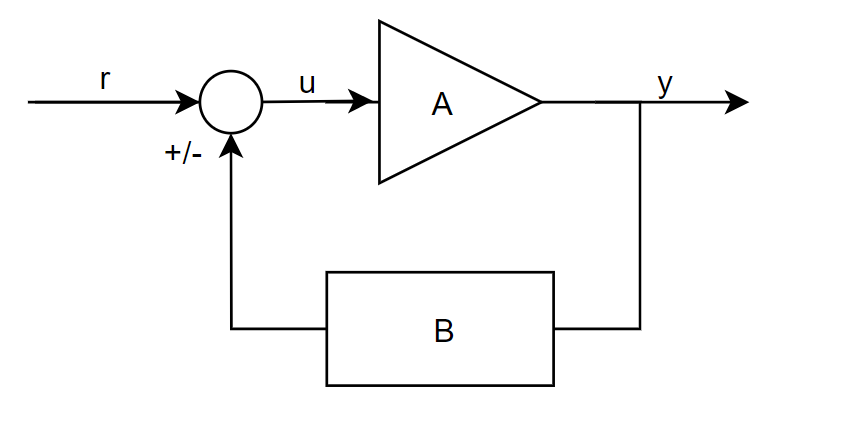
\includegraphics[scale=0.4]{feedback.png}
\caption{Model systemu zamkniętego}
\label{fig:model}
\end{figure}

\subsection{Ze sprzężeniem zwrotnym dodatnim}


\quad Układy takie zwielokrotniają wzmocnienienie sygnału co sprawia, że charakteryzują się niską stabilnością. 
W elektronice takie systemu stosuje się głównie w oscylatorach, których dzieki silnemu sprzężeniu, następuje generacja drgań.
Sprzężenie zwrotne dodatnie wykorzystuje się również w przerzutniku Schmitta, który jest włączany w obwód przekształcający analogowy sygnał wejściowy do cyfrowego sygnału wejściowego.

Codziennym przykładem sprzężenia zwrotnego dodatniego jest sytuacja w której zbliżono do głośnika mikrofon, z którego sygnał jest odtwarzany przez głośnik. Utworzona pętla znacząco wzmacnia sygnał doprowadzając do gwałtownego wzrostu głośności sprawiając, że wydobywający się z głośnika dźwięk staje staje się charakterystycznym piskiem.

\subsection{Ze sprzężeniem zwortnym ujemnym}

\quad Układy tego typu są bardzo często spotykane, charakteryzują się wysoką stabilnością ponieważ umożliwiają łatwe utrzymanie sygnału wyjściowego blisko oczekiwanych wartości. Takie systemy spotyka się nie tylko w elektronice, lecz także w naturze.\\ Prostym przykładem takiego systemu może być populacja drapiezników i ofiar. Gdy liczba drapieżników jest wysoka, maleje liczba osobników zwierząt, na które polują, w wyniku czego drapieżniki zaczynają głodować, a ich populacja się zmniejsza. System sam się reguluje poprzez zmiany w populacjach utrzymując oscylację między stałym poziomem. 

W podobny sposób organizm człowieka reguluje poziom cukru we krwi. 
Gdy poziom ten wzrasta, uwalniana jest insulina obniżająca go, natomiast gdy spadnie zbyt nisko, uwalniana jest glukoza.

W elektronice termostat jest jednym z urządzeń, w których do regulacji temperatury w pomieszczeniu wykorzystywane jest właśnie sprzężenie zwrotne. 
Urządzenie reguluje temperaturę w pomieszczeniu poprzez mierzenie jej i regulowanie ogrzewania w taki sposób by uzyskać oczekiwaną temperaturę w tym samym pomieszczeniu.

W procesorach można się spotkać ze zjawiskiem throttlingu, który ma na celu ograniczenie temperatury rdzenia przez ograniczenie częstotliwości taktowania. 
Układ stara się utrzymać bezpieczną temperaturę pracy jednoczenie zachowując jak najwyższą wydajność. 
Częstotliwość zegara jest regulowana tak by układ nie przekraczał maksymalnej bezpiecznej temperatury.

\end{document}
